\documentclass[UTF8]{ctexart}
\usepackage{amsmath}
\usepackage{amssymb}
\usepackage{background}
\usepackage{booktabs}
\usepackage{caption}
\usepackage{enumitem}
\usepackage{fancyhdr}
\usepackage{float}
\usepackage{fontspec}
\usepackage{geometry}
%\usepackage[bookmarksnumbered = true, pdfborder=0 0 0]{hyperref}
\usepackage{kbordermatrix} % 会标注信息的矩阵
\usepackage{listings}
\usepackage{tasks}
\usepackage{tcolorbox}
\tcbuselibrary{breakable}
\usepackage{tikz}
\usetikzlibrary{arrows.meta, positioning, calc, shapes.geometric}
\usepackage[table]{xcolor}

\geometry{a5paper, top=0.1cm, left=1cm, right=1cm, bottom=1cm, footskip=0.1cm}
\setCJKmainfont[BoldFont={汉仪文黑-85W},ItalicFont={汉仪文黑-55W}]{汉仪文黑-55W}
\setfontfamily\Issue{Century Schoolbook}
\setfontfamily\Genshin{Genshin Teyvat Lingua Franca}
\newCJKfontfamily\TitleFont{思源宋体 CN Heavy}
\newfontfamily\timesnewroman{Times New Roman}

%————————————————可变部分——————————————————
\settasks{label={\Alph*.\ }, label-format={\color{cyan!50!black}}, item-format={\color{cyan!50!black}}}
\newcommand\col[1]{\textcolor{green!50!black}{#1}}
\newcommand\coll[1]{\textcolor{blue}{#1}}
\newcommand\dotting{\ .\ }
\newcommand\pai{\text{\timesnewroman π}}
%\setlist[enumerate]{itemsep=0pt, parsep=0pt}
%\setlist[itemize]{itemsep=0pt, parsep=0pt}
\captionsetup{labelfont=bf, font=small}
\CTEXsetup[format = {\bfseries\color{darkcyan}}]{paragraph}

\lstset{
    language = C,
    basicstyle=\small\ttfamily, %注意行末有逗号!
    keywordstyle=\bfseries\color{blue!70!black},
    commentstyle=\color{cyan!90!black},
    stringstyle=\color{green!40!black},
    columns=flexible,
    numbers=left,
    numberstyle=\footnotesize,
    escapechar=`,
    frame=shadowbox,
    %rulesepcolor=\color{red!20!blue!20!green!20}
    backgroundcolor=\color{cyan!5!white},
    tabsize = 4,
    breaklines = true,
    showstringspaces = false,
}

\newtcolorbox{all-summary}[0]{colback = yellow!20, colframe = brown, boxrule = 1pt}
\newtcolorbox{summary}[1][章节内容梗概]{colback = cyan!10, colframe = cyan!80, boxrule = 1pt, title = {#1}}
%——————————————————————————————————————————

\pagestyle{fancy}
\fancyhf{}
\cfoot{\sffamily\footnotesize{-\ \thepage\ -}}
%

\colorlet{darkcyan}{cyan!50!black}
\newcommand\Black[1]{\textcolor[gray]{0.3}{#1}}
\newcommand\Brown[1]{\textcolor[HTML]{998A4E}{#1}}
\newcommand\Emph[1]{\textcolor{cyan!80!black}{#1}}
\newcommand\Notes[1]{\textcolor{yellow!50!black}{\small #1}}
\newcommand\Example[1]{\textcolor{cyan!70!black}{\small #1}}
\colorlet{note}{yellow!70!black}


\newcommand\IssueNumber{48}
\newcommand\Date{2025-1-3}
%\newcommand\Contributer{@金光日}
\newcommand\Subject{算法分析与设计}
%\newcommand\Source{历年考研 408 真题}


\begin{document}
\backgroundsetup{contents=\includegraphics{上半示例.png}, center, scale=1, angle=0, opacity=1}
\BgThispage
\begin{center}
%{\scriptsize\Issue \textcolor[HTML]{C8BA83}{\Genshin WEEKLY TIPS}}
\phantom{...}

{\Large\textcolor{brown!40!white}{\makebox[10cm][s]{\Genshin WEEKLY KNOWLEDGE TIPS}}}

\vspace{-2em}

{\Huge\bfseries\TitleFont \Black{知\ 识\ 小\ 料}}


\vspace{-0.1cm}
{\footnotesize \Brown{「电计 2203 班」周常规知识整理共享}}
\end{center}

\vspace{-0.5cm}


\begin{figure}[H]
\hspace{1cm}
\begin{minipage}[t]{0.3\textwidth}
\centering
    \Brown{\Genshin ISSUE}

    \vspace{-0.6cm}
    \Huge \Issue\slshape\bfseries\Black{\IssueNumber}
\end{minipage}
\hfill
\begin{minipage}[t]{0.35\textwidth}
\centering
    \Brown{日期:\Date} \\
%\vspace{-0.1cm}
%    \Brown{贡献者:\Contributer} \\
\vspace{-0.1cm}
    \Brown{学科:\Subject} \\
%\vspace{-0.1cm}
%    \Brown{来源:\Source}
\end{minipage}
\hspace{0.8cm}
\end{figure}

{\color{darkcyan}本文档用于对《算法分析与设计》本科选修课(不是研究生课程)进行简明复习。}

\begin{all-summary}
\begin{itemize}[itemsep=0pt,parsep=0pt]
  \item 第 1 章:算法复杂度分析,熟悉各种算法的时间复杂度
  \item 第 2 章:全
  \item 第 3 章:全
  \item 第 4 章:活动安排问题、最优装载问题、单源最短路径问题、最小生成树
  \item 第 5 章:全
  \item 第 6 章:6.1, 6.2 章节
\end{itemize}

【编程重点】最大子段和、最优装载、0-1背包、LCS(最长公共子序列)、活动安排问题、棋盘覆盖问题、多边形游戏。(下文中属于这一类的算法都会在「章节内容梗概」中\Emph{高亮}显示。)
\end{all-summary}

\section{算法绪论}
程序 = 算法 + 数据结构。

关于算法:算法的特征、算法的描述、算法设计。

算法的时间复杂性:最坏、最好、平均。

复杂度:$O(1) < O(\log N) < O(N) < O(N\log N) < O(N^2) < O(N^3) < O(2^N) < O(N!)$

短语句算法复杂度分析:
\begin{enumerate}[itemsep=0pt,parsep=0pt,leftmargin=1.5cm]
  \item 顺序:各个语句计算时间直接相加
  \item 条件:取两个分支的较长时间者
  \item 循环:循环体内时间$\times$ 循环次数
  \item 嵌套循环:循环体内时间$\times$ \Emph{所有}循环次数
\end{enumerate}

「最优算法」:计算时间复杂性等于计算时间下界的算法,如堆排序。

NP 问题相关概念。


\section{递归与分治}

\backgroundsetup{contents=\includegraphics{空白示例.png}, center, scale=1, angle=0, opacity=1}
\BgThispage
\begin{summary}
递归算法:直接或间接地调用自身的算法。递归函数两要素:边界、递归方程。
\begin{enumerate}[itemsep=0pt,parsep=0pt]
  \item 阶乘函数
  \item 斐波那契(Fibonacci)数列
  \item 阿克曼(Ackermann)函数
  \item 排列问题
  \item 整数划分问题
  \item 汉诺塔(Hanoi)问题
\end{enumerate}
\tcblower
分治与二分。
\begin{enumerate}[itemsep=0pt,parsep=0pt]
  \item 大整数乘法
  \item Strassen矩阵乘法
  \item \Emph{棋盘覆盖问题}
  \item 归并排序
  \item 快速排序
  \item 线性时间选择
  \item 最接近点对问题
  \item 循环赛日程表
\end{enumerate}
\end{summary}

\subsection{递归算法}

递归算法是直接或者间接调用自身的算法,其对应函数称为递归函数。递归函数有两个要素——边界条件、递归方程。

\paragraph{阶乘函数}
\begin{equation*}
    n! = \begin{cases}
           1, & n=0\text{\quad(边界条件)}\\
           n\cdot (n-1)! & n>0\text{\quad(递归方程)}
         \end{cases}
\end{equation*}

\paragraph{斐波那契数列}
\begin{equation*}
    F(n) = \begin{cases}
           1, & n=0,1\text{\quad(边界条件)}\\
           F(n-1)+F(n-2) & n>1\text{\quad(递归方程)}
         \end{cases}
\end{equation*}

\paragraph{阿克曼函数}
\begin{equation*}
    A(n,m) = \begin{cases}
           2, & n=1,m=0\text{\quad(边界条件)}\\
           1, & n=0,m\geqslant 0\text{\quad(边界条件)}\\
           n+2, & n\geqslant 2,m=0\text{\quad(递归方程)}\\
           A(A(n-1,m),m-1) & n,m\geqslant 1\text{\quad(递归方程)}
         \end{cases}
\end{equation*}

\begin{itemize}
  \item 固定 $m$ 时,对应的一元函数 $A(n,0)=n+2$,$A(n,1)=2n$,$A(n,2)=2^n$……阿克曼函数增长速度十分迅速。
  \item 单变量阿克曼函数 $A(n) := A(n,n)$。
  \item 反阿克曼函数 $\alpha(n) := \min\{k | A(k)\geqslant n\}$。对于 $\forall n\leqslant 2^{2^{2^{65536}}}-3$,$\alpha(n)\leqslant 4$。
\end{itemize}

\paragraph{排列问题}
集合 $R=\{r_1,r_2,\dots,r_n\}$ 的全排列可以用如下定义进行递归表示,记为 $perm(R)$。
\begin{enumerate}
  \item 边界条件:$n=1$ 时,$perm(R) = (r_1)$。
  \item 递归函数:$n>1$ 时,$perm(R)$ 由 $(r_1)perm(R_1)$、$(r_2)perm(R_2)$、$\dots$、$(r_n)perm(R_n)$ 构成。
\end{enumerate}
其中,$R_i = R - \{r_i\}$。

\paragraph{整数划分问题}
定义 $q(n,m)$ 为正整数 $n$ 的最大加数不大于 $m$ 的划分数量。
\begin{equation*}
    q(n,m) = \begin{cases}
           1, & m=1\ \text{或}\ n=1\text{\quad(边界条件)}\\
           q(n,n), & m>n\geqslant 0\text{\quad(递归方程)}\\
           1 + q(n,n-1), &m=n  \text{\quad(递归方程)}\\
           q(n,m-1) + q(m-n,m), &m<n  \text{\quad(递归方程)}
         \end{cases}
\end{equation*}

\paragraph{汉诺塔问题}
将 $n$ 个圆盘挪 $a\to b$,以 $c$ 为中转塔座,每次挪一个,且必须保持小圆盘在大圆盘上方。设 $Hanoi(n,a,b,c)$ 表示上述场景的移动。

\begin{enumerate}
  \item 递归函数:当 $n>0$ 时,先将 $n-1$ 个圆盘挪 $a\to c$,然后将最底下 1 个圆盘挪 $a\to b$,随后将刚才的 $n-1$ 个圆盘挪 $c\to b$。
  \item 边界条件:当 $n=0$ 时,结束,返回。
\end{enumerate}

\subsection{分治算法}
分治即是分而治之,将同一问题分为多个相互独立的子问题,解决后合并。二分是其中一种分治。

\paragraph{大整数乘法}
假设有两个 $n$ 位二进制大整数 $X=[ab],Y=[cd]$,其中 $a,b,c,d$ 都是 $\frac n2$ 位,今需计算 $XY$。

\begin{itemize}
  \item 第一种分治:$XY = ac\cdot 2^n + (ad+bc)\cdot 2^{\frac{n}{2}} + bd$。计算四次乘法:$ac,ad,bc,bd$。
  \item 第二种分治:$XY = ac\cdot 2^n + (\textcolor{green!50!black}{(a-b)(d-c) + ac + bd})\cdot 2^{\frac n2} + bd$。计算三次乘法:$ac,bd,(a-c)(b-d)$。
\end{itemize}
第二种分治更优。\Emph{时间复杂度 $O(n^{1.59})$。}

\paragraph{Strassen矩阵乘法}
假设有两个矩阵 $A=\begin{bmatrix}
             A_{11} & A_{12} \\
             A_{21} & A_{22}
           \end{bmatrix}$,$B=\begin{bmatrix}
                               B_{11} & B_{12} \\
                               B_{21} & B_{22}
                             \end{bmatrix}$,今需计算 $C=AB$。
平时的矩阵乘法是 $O(n^3)$。

这种方法计算了 7 个中间矩阵 $M_1\sim M_7$(其中幻灯片被挡住的部分 $M_1=A_{11}(B_{12}-B_{22})$),然后计算中间 $C_{11},C_{12},C_{21},C_{22}$,拼成答案 $C$。\Emph{时间复杂度 $O(n^{2.81})$。}

\paragraph{棋盘覆盖问题}
当 $k>0$ 时,将 $2^k\times 2^k$ 棋盘划分为 4 个 $2^{k-1}\times 2^{k-1}$ 的子棋盘。在调用函数时,如果特殊方格在某个子棋盘中,则在递归时沿用特殊方格的位置;如果不在该子棋盘中,则在递归时将特殊方格的位置记在相应的一角处。

时间复杂度 $O(4^k)$。

\begin{figure}
    \centering
    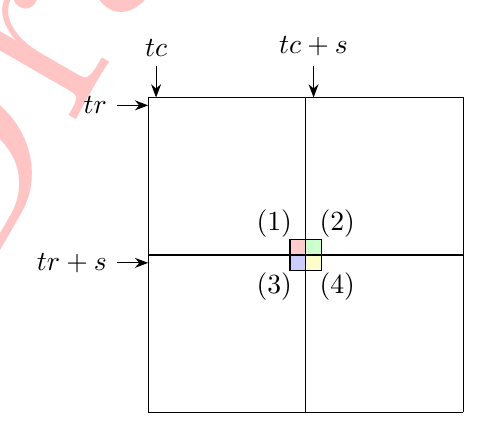
\begin{tikzpicture}[scale=2,>=Stealth]
        \draw (0,0) grid (2,2);
        \coordinate (tr+s) at (0, 0.95);
        \coordinate (tr) at (0, 1.95);
        \coordinate (tc) at (0.05, 2);
        \coordinate (tc+s) at (1.05, 2);
        \draw [->] ($(tr)+(-0.2,0)$) node[left] {$tr$} -- (tr) ;
        \draw [->] ($(tr+s)+(-0.2,0)$) node[left] {$tr+s$} -- (tr+s);
        \draw [->] ($(tc)+(0,0.2)$) node[above] {$tc$} -- (tc);
        \draw [->] ($(tc+s)+(0,0.2)$) node[above] {$tc+s$} -- (tc+s);
        \filldraw[fill=red!20] (0.9, 1) rectangle (1, 1.1) node at (0.8, 1.2) {(1)};
        \filldraw[fill=green!20] (1, 1) rectangle (1.1, 1.1) node at (1.2, 1.2) {(2)};
        \filldraw[fill=blue!20] (0.9, 0.9) rectangle (1, 1) node at (0.8, 0.8) {(3)};
        \filldraw[fill=yellow!20] (1, 0.9) rectangle (1.1, 1) node at (1.2, 0.8) {(4)};
    \end{tikzpicture}
    \caption{棋盘格子指示}\label{fig:chess-board}
\end{figure}

读代码时,值得注意几个对角格的位置:
\begin{enumerate}[label = {(\theenumi):\quad}, itemsep=0pt,parsep=0pt]
  \item $(tr+s-1, \quad tc+s-1)$
  \item $(tr+s-1, \quad tc+s)$
  \item $(tr+s,\quad  tc+s-1)$
  \item $(tr+s, \quad tc+s)$
\end{enumerate}

\paragraph{归并排序} 老生常谈的排序方法。将待排序元素分成两个子集合,分别递归地排序,随后合并两个子集合。\Emph{时间复杂度 $O(n\log n)$。}

\paragraph{快速排序} 老生常谈的排序方法。每次排序后,小于枢轴的数位于枢轴左侧,大于枢轴的数位于枢轴右侧。\Emph{时间复杂度平均 $O(n\log n)$,最坏 $O(n^2)$。}

\paragraph{线性时间选择} 选出 $n$ 个元素中第 $k$ 小的元素。主要步骤如下:
\begin{enumerate}[itemsep=0pt,parsep=0pt]
  \item 选择一个元素作为基准值。
  \item 类似快速排序,将数据分成两部分,比基准值小的放在左侧,大的放在右侧。
  \item 通过基准值的位置是否在第 $k$ 位进行递归查找:恰在第 $k$ 位则结束,位置大于第 $k$ 位则递归查找左侧,小于第 $k$ 位则递归查找右侧。
\end{enumerate}

其优化在于选择基准值。可以随机选取,也可以选取「中位数」:
\begin{enumerate}[itemsep=0pt,parsep=0pt]
  \item 把 $n$ 个元素分为 $\frac n5$ 组,每组 5 个元素,通过少量比较选出每一组的中位数。
  \item 递归地使用上述过程找出 $\frac n5$ 个元素的中位数,直到找出唯一的中位数。
\end{enumerate}
可以证明这种选取中位数的方法是 $O(n)$ 的。整个算法\Emph{时间复杂度 $O(n)$。}

\paragraph{最接近点对问题} 对于一维情形:
\begin{itemize}
  \item 分治:取中位点 $m$ 将原集合划分为两子集 $S_1,S_2$,递归地求出两个子集内部的最接近点对,距离记为 $d$。
  \item 合并:$S$ 的最接近点对距离要么是 $d$,要么是 $S_1$ 的某个点与 $S_2$ 的某个点的距离(记为 $\{p_3,q_3\}$),取二者较小值。
  \item 可以证明:$p_3$ 一定是 $S_1$ 中坐标最大的点,$q_3$ 一定是 $S_2$ 中坐标最小的点。
\end{itemize}

{\noindent 对于二维情形:}
\begin{itemize}
  \item 分治:取垂直线 $x=m$ 将原集合划分为两子集 $S_1,S_2$,递归地求出两个子集内部的最接近点对,距离记为 $d$。
  \item 合并:$S$ 的最接近点对距离要么是 $d$,要么是 $S_1$ 的某个点与 $S_2$ 的某个点的距离(对于 $P_1$ 区域中任一点 $p$,检查位于 $P_2$ 区域的 $d\times 2d$ 矩形的至多 6 个点),取二者较小值。
  \item 可以证明:对于 $P_1$ 区域中任一点 $p$,可能触发归并的 $P_2$ 区域的点必然落在 $d\times 2d$ 矩形内。
  \item 其中:$P_1,P_2$ 分别是垂直线 $x=m$ 左、右两侧的宽为 $d$ 的垂直长条。
\end{itemize}

一维和二维问题的\Emph{时间复杂度均为 $O(n\log n)$。}

\paragraph{循环赛日程表} 
\begin{itemize}
  \item 递归函数:将所有 $n$ 名选手分成两半,递归地处理每一半。合并时,将日程表左上部映像到右下部,左下部映像到右上部即可。
  \item 边界条件:当 $n=2$ 时,手动指定两名选手的日程表即可。
\end{itemize}
幻灯片中给出的是递推思路的代码。\Emph{时间复杂度 $O(n^2)$。}

\section{动态规划}
\begin{summary}
动态规划问题会记录已解决的子问题的答案。需要满足最优子结构性质。
\begin{enumerate}[itemsep=0pt,parsep=0pt]
  \item 矩阵连乘积
  \item \Emph{最长公共子序列}
  \item \Emph{最大子段和}
  \item 凸多边形的最优三角剖分
  \item \Emph{多边形游戏}
  \item 电路布线问题
  \item 流水作业调度问题·动态规划法(含Johnson不等式)
  \item \Emph{0-1背包问题·动态规划法}
  \item 最优二叉搜索树
\end{enumerate}
\end{summary}

动态规划(DP)算法与分治类似,都需要把问题划分为子问题求解。不同之处是动态规划求解的子问题有依赖性,可以通过记下已求解的子问题答案来避免重复求解,提高效率。

动态规划算法的基本要素:最优子结构性质、重叠子问题性质,采用备忘录方法。

\paragraph{矩阵连乘积} 给定 $n$ 个可连乘的矩阵 $A_1A_2\cdots A_n$,需要利用结合律,确定最优的求解顺序(加括号顺序),使得做乘法的次数最少。

\begin{itemize}
  \item 在求解大矩阵 $A_i A_{i+1}\cdots A_j$ 时,可以考虑选择恰当的点 $k$,在此处将矩阵断开为 $(A_i A_{i+1}\cdots A_k)\cdot (A_{k+1}\cdots A_j)$,随后递归地求解小矩阵 $A_i A_{i+1}\cdots A_k$ 和 $A_{k+1}\cdots A_j$。
  \item 这启示我们,可以先计算规模较小的子问题,这样当我们遇到规模较大的子问题时,就可以直接使用记录好的规模较小的子问题的答案,避免重复计算。这里的「规模」指连乘的矩阵个数(即 $j-i+1$)。
\end{itemize}

建立递归关系:
\begin{itemize}[itemsep=0pt,parsep=0pt]
  \item 设求解子问题 $A_i A_{i+1}\cdots A_j$ 的最少乘法次数为 $m[i,j]$($1\leqslant i\leqslant j\leqslant n$)。
  \item 当 $i=j$ 时,单个矩阵不需相乘,$m[i,i]=0$。
  \item 当 $i<j$ 时,我们的子问题结果为
  \begin{enumerate}[itemsep=0pt,parsep=0pt]
    \item 子问题 $A_i A_{i+1}\cdots A_k$ 的乘法次数:$m[i,k]$
    \item 加上子问题 $A_{k+1}\cdots A_j$ 的乘法次数:$m[k+1,j]$
    \item 加上两大矩阵合并时计算的乘法次数:$p_{i-1} p_k p_j$ \textcolor{cyan}{(注:矩阵 $A_{m\times n}$ 和 $B_{n\times p}$ 相乘时的乘法次数为 $m\cdot n\cdot p$。)}
  \end{enumerate}
  \item 选择 $k$ 时,遍历 $k\in [i,j)$,取达到最少乘法次数的那一个值。
\end{itemize}

状态转移方程:
\begin{equation*}
    m[i,j] = \begin{cases}
               0, & i=j \\
               \min\limits_{i\leqslant k<j} \{m[i,k] + m[k+1,j] + p_{i-1}p_kp_j\}, & i<j 
             \end{cases}
\end{equation*}

在代码中,辅以数组 $s[i,j]$ 表示记录断开位置。\Emph{时间复杂度 $O(n^3)$。}

\paragraph{最长公共子序列(LCS)} 设序列 $X$ 的前 $i$ 个元素的子序列为 $X_i$,设序列 $X_i,Y_j$ 的最长公共子序列的长度为 $c[i,j]$。

\begin{itemize}
  \item 当 $i=0$ 或 $j=0$ 时,$X_i,Y_j$ 的其中一个序列为空,$c[i,j]=0$。
  \item 当 $x_i=y_j$ 时,说明 $c[i,j]$ 恰好可以由 $c[i-1,j-1]$ 添加一个元素得到。
  \item 当 $x_i\ne y_j$ 时,说明 $c[i,j]$ 可以由 $c[i,j-1]$ 或 $c[i-1,j]$ 的较大者转移得来。
\end{itemize}

状态转移方程:
\begin{equation*}
  c[i,j] = \begin{cases}
             0, & i=0\text{\ 或\ }j=0 \\
             c[i-1,j-1] + 1, & x_i = y_j \\
             \max\{c[i,j-1],\quad c[i-1,j]\}, & x_i\ne y_j 
           \end{cases}
\end{equation*}
\Emph{时间复杂度 $O(n^2)$。}

\paragraph{最大子段和·分治算法}
将大序列 $a[1\sim n]$ 分成两段小序列:$a[1\sim \frac n2]$ 和 $a[\frac n2+1\sim n]$。在合并时,大序列的最大子段和要么与其中一个小序列的相等,要么横跨两个小序列。对于后者,可以事先算出 $s_1 = \max\limits_{i} \{a_i + a_{i+1} + \cdots + a_{\frac{n}{2}}\}$,$s_2 = \max\limits_{i} \{a_{\frac{n}{2}+1} + \cdots + a_{i-1} + a_i\}$,则最优值为 $s_1+s_2$。\Emph{时间复杂度 $O(n\log n)$。}

\paragraph{最大子段和·动态规划算法}
记 $b[j] = \max\limits_{i\in [1,j]} \{a_i + a_{i+1} + \cdots + a_j\}$(其中 $1\leqslant j\leqslant n$),也就是固定以下标 $j$ 结尾的最大子段和。则答案为 $\max\limits_j b[j]$。

对 $b[j]$ 的递推也就是「继承结果」和「另起炉灶」的区别:
\begin{equation*}
    b[j] = \max\{b[j-1]+a[j], \quad a[j]\}, \quad 1\leqslant j\leqslant n
\end{equation*}

$j$ 从 1 到 $n$ 直接遍历即可得到答案。\Emph{时间复杂度 $O(n)$。}

\paragraph{凸多边形的最优三角剖分} 该问题类似于\Emph{矩阵连乘积}问题,关键在于找到断开点的位置。

\begin{itemize}
  \item 定义:设 $t[i,j]$ 表示凸多边形 $\{v_{i-1}, v_i, \dots, v_j\}$ 的最优解(最优剖分对应的权函数值)。规定退化为线段的「凸二边形」$\{v_{i-1},v_i\}$ 的最优解 $t[i,i]=0$。
  \item 转移:求解大的凸多边形 $\{v_{i-1}, v_i, \dots, v_j\}$ 时,考虑找到恰当的点 $k$,将大的凸多边形划分成两个小的凸多边形 $\{v_{i-1}, v_i,\dots, v_k\}$ 和 $\{v_k, \cdots, v_j\}$。
\end{itemize}

状态转移方程:
\begin{equation*}
  t[i,j] = \begin{cases}
             0, & i=j \\
             \max\limits_{i\leqslant k <j} \{t[i,k] + t[k+1,j] + w(v_{i-1} v_k v_j)\}, & i<j \\
           \end{cases}
\end{equation*}
其中 $w(v_{i-1} v_k v_j)$ 是三角形 $\{v_{i-1},v_k,v_j\}$ 对应的权函数值。\Emph{时间复杂度 $O(n^3)$。}

\paragraph{多边形游戏} 

\begin{itemize}
  \item 设 $p(i,j)$ 表示从顶点 $v_i$ 开始一直持续了 $j$ 个顶点的一条链\textcolor{cyan}{(如 $p(i,3)$ 表示 $v_i-op_{i+1}-v_{i+1}-op_{i+2}-v_{i+2}$)},设 $m[i,j,0/1]$ 表示链 $p(i,j)$ 合并的最小(0)/最大(1)值。
  \item 考虑在 $s$ 处断开,把大链 $p(i,j)$ 断成两个小链 $p(i,s)$ 和 $p(i+s,j-s)$。那么大链的解便可以由小链转移得来。
  \item 设两条小链的值 $a=m[i,s,0]$,$b=m[i,s,1]$,$c=m[i+s,j-s,0]$,$d=m[i+s,j-s,1]$,则对于每个特定的断开点 $s$,状态转移方程如下:
\end{itemize}
\begin{equation*}
    \mathrm{minf}(i,j,s) = \begin{cases}
                 a+c, & op_{i+s}\text{\ 为加号} \\
                 \min\{ac,ad,bc,bd\}, &op_{i+s}\text{\ 为乘号} 
               \end{cases}
\end{equation*}
\begin{equation*}
    \mathrm{maxf}(i,j,s) = \begin{cases}
                 b+d, & op_{i+s}\text{\ 为加号} \\
                 \max\{ac,ad,bc,bd\}, &op_{i+s}\text{\ 为乘号}
               \end{cases}
\end{equation*}
\begin{equation*}
\begin{aligned}
    m[i,j,0] &= \min\limits_{1\leqslant s<j} \{\mathrm{minf}(i,j,s)\} \\
    m[i,j,1] &= \max\limits_{1\leqslant s<j} \{\mathrm{maxf}(i,j,s)\}
\end{aligned}
\end{equation*}

边界条件:$m[i,1,0] = m[i,1,1] = v_i$。

于是最终答案为 $\max\limits_{i} m[i,n,1]$,\Emph{时间复杂度 $O(n^3)$。}

\paragraph{电路布线} 给定 $n$ 条导线,每条导线分别连接 $i$ 和 $\pai(i)$ 两点,现需求出导线集合的最大不交叉子集。例如幻灯片上的 $\{(3,4), (5,5), (7,9), (9,10)\}$ 可能是最大不交叉子集(目测)。

\begin{itemize}
  \item 记 $N(i,j)$ 是上端编号不超过 $i$,下端编号不超过 $j$ 的那些导线的集合。$MNS(i,j)$ 是 $N(i,j)$ 是最大不交叉子集。$Size(i,j)$ 是最大不交叉子集的元素个数。
  \item 当 $i=1$ 时,$N(1,j)$ 导线上端编号只能是 1。若 $j<\pai(1)$,则 $N(1,j)=\varnothing$;若 $j\leqslant \pai(1)$,则 $N(1,j) = \{(1,\pai(1))\}$。
  \item 当 $i>1$ 时,
  \begin{itemize}[itemsep=0pt,parsep=0pt]
    \item 若 $j<\pai(i)$,则导线 $(i,\pi(i))\notin N(i,j)$,因而 $N(i,j)$ 只能由 $N(i-1,j)$ 转移而来,此时 $Size(i,j) = Size(i-1,j)$。
    \item 若 $j\geqslant \pai(i)$,则导线 $(i,\pi(i))\in N(i,j)$。可以证明,$Size(i,j)$ 等于 $Size(i-1,j)$ 或 $Size(i-1,\  \pai(i)-1)+1$ 的较大者。
  \end{itemize}
\end{itemize}
\begin{equation*}
  Size(i,j) = \begin{cases}
                Size(i-1,j), & j<\pai(i) \\
                \max\{Size(i-1,j),\quad Size(i-1,\ \pai(i)-1)+1\}, &j\geqslant \pai(i) 
              \end{cases}
\end{equation*}
\begin{equation*}
  Size(1,j) = \begin{cases}
                0, & j<\pai(1) \\
                1, & j\geqslant \pai(1)
              \end{cases}
\end{equation*}
\Emph{时间复杂度$O(n^2)$。}

\paragraph{流水作业调度问题} $n$ 个作业要先后在两个机器完成加工后才能出厂,每个作业 $i$ 在两台机器的加工时间分别为 $a_i,b_i$,每台机器至多加工一个作业,现需找到最少的总加工时间。

有相互等价的两个版本的算法方案,以下是版本 A:
\begin{enumerate}[itemsep=0pt,parsep=0pt]
  \item 令 $N_1 = \{i|a_i<b_i\}$,$N_2 = \{i|a_i\geqslant b_i\}$。
  \item 将 $N_1$ 的元素按 $a$ 值从小到大排列,将 $N_2$ 的元素按 $b$ 值从大到小排列。
  \item 最优调度顺序就是 $N_1$ 顺序接着 $N_2$ 的顺序。
\end{enumerate}

版本 B:
\begin{enumerate}[itemsep=0pt,parsep=0pt]
  \item 对全部的 $\{a_i\},\{b_i\}$ 从小到大排列,按 $a,b$ 值交替加入序列 $S$;设调度数组为 $job$,初始为空。
  \item 如果 $S$ 的下一个数是 $a_i$,则把任务 $i$ 放在 $job$ 的最左侧;如果下一个数是 $b_i$,则把任务 $i$ 放在 $job$ 的最右侧。随后 $S$ 删除 $\{a_i,b_i\}$。
  \item 最优调度顺序就是 $job$ 数组。
\end{enumerate}

通过上述方案得到的最优调度顺序 $S$,对于 $i<j$,总有 $\min\{b_i,a_j\}\geqslant \min\{b_j,a_i\}$,也就是序列 $S$ 中任意两个元素均满足 Johnson 不等式。\Emph{时间复杂度主要在于排序:$O(n\log n)$。}

\paragraph{0-1背包问题} 给定 $n$ 个物品,第 $i$ 个物品有重量 $w_i$ 和价值 $v_i$;给定容量为 $C$ 的背包,问如何装载物品使得物品不超过最大容量且总价值最大?

\begin{itemize}
  \item $m(i,j)$ 为可选择物品有 $\{i,i+1,\dots,n\}$,背包容量为 $j$ 时的子问题的最优值。
  \item 外层对 $i$ 循环,内层对 $j$ 循环。考虑第 $i$ 个物品,
  \begin{enumerate}[itemsep=0pt,parsep=0pt]
    \item 当第 $i$个物品装不下时,$m(i,j)$就等于 $m(i+1,j)$;
    \item 当第 $i$ 个物品能装下时,$m(i,j)$就等于 $\max\{m(i+1, j),\quad m(i+1, j-w_i)+v_i \}$。
  \end{enumerate}
\end{itemize}

状态转移方程:
\begin{equation*}
    m(i,j) = \begin{cases} 
    \max\{m(i+1, j),\quad m(i+1, j-w_i)+v_i \} &w_i\leqslant j \\ m(i+1,j) & w_i > j
    \end{cases}
\end{equation*}

初始值:对所有的 $j\in [0,C]$ 初始化如下
\begin{equation*}
    m(n,j) = \begin{cases}  v_n & w_n\leqslant j \\ 0 & w_n > j \end{cases}
\end{equation*}

答案:$m(1,C)$。\Emph{时间复杂度 $O(\min\{nC,2^n\})$。}

\paragraph{最优二叉搜索树} 

\begin{itemize}
  \item 假设 $T_{ij}$ 是关于点 $\{x_i,x_{i+1},\dots,x_j\}$ 的最优二叉搜索树,$p_{ij}$ 是 $T_{ij}$ 的平均路长,$w_{ij}$ 是诸概率之和,$m(i,j) = p_{ij}\cdot w_{ij}$。
  \item 考虑选 $k$ 为根结点断开,将大树分成 $m(i,k-1)$ 左子树和 $m(k+1,j)$ 为右子树。
\end{itemize}
状态转移方程:
\begin{equation*}
  m(i,j) = w_{ij} + \min\limits_{i\leqslant k\leqslant j} \{m(i,k-1) + m(k+1,j)\}\qquad (i\leqslant j)
\end{equation*}
边界:$m(i,i-1)=0$。

辅以数组 $s[i,j]$ 保存树 $T_{ij}$ 的根结点。整个最优二叉搜索树的根结点为 $s[1,n]$。\Emph{时间复杂度 $O(n^2)$。}

\section{贪心算法}
\begin{summary}
贪心算法做出来的只是当前局面的局部最优选择。
\begin{enumerate}[itemsep=0pt,parsep=0pt]
  \item \Emph{活动安排问题}
  \item 0-1背包问题·贪心算法(不可用)
  \item \Emph{最优装载问题}
  \item 哈夫曼(Huffman)编码
  \item 单源最短路径·Dijkstra算法
  \item 最小生成树·Kruskal和Prim算法
  \item 多机调度问题
  \item 贪心算法理论基础(略)
\end{enumerate}
\end{summary}


\section{回溯算法}
\begin{summary}
回溯算法按照深度优先搜索策略搜索,用递归方式实现。
\begin{enumerate}[itemsep=0pt,parsep=0pt]
  \item \Emph{最优装载问题}
  \item 流水作业调度问题·回溯法
  \item 符号三角形问题
  \item $n$ 皇后问题
  \item \Emph{0-1背包问题·回溯法}(效率过低)
  \item 最大团问题
  \item 图的 $m$ 着色问题
  \item 旅行售货员问题
  \item 圆排列问题
  \item 连续邮资问题
  \item 重排原理
\end{enumerate}
\end{summary}

\section{概率算法}

\begin{summary}
概率算法是带有一定概率成功找到正确解的算法。
\begin{enumerate}[itemsep=0pt,parsep=0pt]
  \item 伪随机数产生
  \item 随机投点法计算圆周率
  \item 随机投点法、平均法计算定积分
  \item 几种概率算法的对比
\end{enumerate}

\end{summary}

\backgroundsetup{contents=\includegraphics{下半示例.png}, center, scale=1, angle=0, opacity=1}
\BgThispage

\end{document} 